% =====================================================================
%  POLISHED PDF — house visual style (reusable LaTeX template)
%  Engine: XeLaTeX via Tectonic.   Build:  tectonic -X compile doc.tex
%  Fonts come from the TeX Live bundle (Tectonic auto-downloads them):
%  NO system fonts required, so it builds identically on any machine.
% =====================================================================
\documentclass[12pt,a4paper]{article}   % 12pt = "spacious / Preset A". Use 11pt for denser.

% ---------- fonts: TeX Gyre Pagella (Palatino) body, Heros (Helvetica) headings ----------
\usepackage{fontspec}
\setmainfont{texgyrepagella-regular.otf}[
  BoldFont=texgyrepagella-bold.otf, ItalicFont=texgyrepagella-italic.otf,
  BoldItalicFont=texgyrepagella-bolditalic.otf]
\setsansfont{texgyreheros-regular.otf}[Scale=0.92,
  BoldFont=texgyreheros-bold.otf, ItalicFont=texgyreheros-italic.otf,
  BoldItalicFont=texgyreheros-bolditalic.otf]
\setmonofont{texgyrecursor-regular.otf}[Scale=0.88, BoldFont=texgyrecursor-bold.otf]

\usepackage{microtype}
\usepackage[a4paper,margin=2.2cm,bottom=2.4cm]{geometry}
\usepackage{xcolor}\usepackage{amsmath}\usepackage{booktabs}
\usepackage{tabularx}\usepackage{array}\usepackage{graphicx}\usepackage{enumitem}
\setlist{itemsep=2pt,topsep=3pt,parsep=0pt}

% ---------- SPACING (default: v1.1-like density at 12pt, a hair of breathing room) ----------
% Inter-block spacing is deliberately tight. For an airier look bump the two values noted below.
\usepackage{setspace}\setstretch{1.07}            % line spacing (1.0 = tightest; 1.15 = airy)
\setlength{\parskip}{0.35\baselineskip}           % space between paragraphs/blocks (0.7 = airy)
\setlength{\parindent}{0pt}                        % no first-line indent (pairs with parskip)
\renewcommand{\arraystretch}{1.08}                 % table rows

% ---------- palette ----------
\definecolor{ink}{HTML}{1A2433}\definecolor{deepblue}{HTML}{14285A}
\definecolor{midblue}{HTML}{1E3C78}\definecolor{accent}{HTML}{2E6FB7}
\definecolor{rule}{HTML}{B4C3DC}\color{ink}
\definecolor{cTheoryBg}{HTML}{E8F0FE}\definecolor{cTheoryFr}{HTML}{4285F4}
\definecolor{cSysBg}{HTML}{E6F4EA}\definecolor{cSysFr}{HTML}{34A853}
\definecolor{cTradeBg}{HTML}{FEF7E0}\definecolor{cTradeFr}{HTML}{F9AB00}
\definecolor{cMathBg}{HTML}{F3E8FD}\definecolor{cMathFr}{HTML}{A142F4}
\definecolor{cFunBg}{HTML}{E0F7FA}\definecolor{cFunFr}{HTML}{12B5CB}
\definecolor{cFailBg}{HTML}{FCE8E6}\definecolor{cFailFr}{HTML}{EA4335}
\definecolor{cProjBg}{HTML}{EFF7E6}\definecolor{cProjFr}{HTML}{7CB342}
\definecolor{cCheckBg}{HTML}{F1F3F4}\definecolor{cCheckFr}{HTML}{80868B}
\definecolor{cNoteBg}{HTML}{F1F3F4}\definecolor{cNoteFr}{HTML}{5F6368}
\definecolor{cMindBg}{HTML}{E3F2FD}\definecolor{cMindFr}{HTML}{1E88E5}   % mental model
\definecolor{cMisBg}{HTML}{FDECEA}\definecolor{cMisFr}{HTML}{D93025}     % misconception
\definecolor{cNoticeBg}{HTML}{EDE7F6}\definecolor{cNoticeFr}{HTML}{673AB7}% notice-this
\definecolor{cAdvBg}{HTML}{ECEFF1}\definecolor{cAdvFr}{HTML}{546E7A}     % advanced (optional depth)
\definecolor{cCompBg}{HTML}{E8F5E9}\definecolor{cCompFr}{HTML}{2E7D32}   % compression / takeaways

% ---------- callout boxes ----------
\usepackage[most]{tcolorbox}
\tcbset{calloutbase/.style={enhanced,breakable,left=3mm,right=3mm,top=2mm,bottom=2mm,
  boxrule=0pt,leftrule=2.2pt,arc=2pt,outer arc=2pt,fonttitle=\sffamily\bfseries\small,
  coltitle=ink,attach title to upper,after title={\par\smallskip},boxsep=1.1mm,
  before skip=6pt,after skip=6pt}}
% --- content-classification boxes ---
\newtcolorbox{theory}[1][Theory]{calloutbase,colback=cTheoryBg,colframe=cTheoryFr,title={#1}}
\newtcolorbox{system}[1][In the System]{calloutbase,colback=cSysBg,colframe=cSysFr,title={#1}}
\newtcolorbox{tradeoff}[1][Engineering Tradeoff]{calloutbase,colback=cTradeBg,colframe=cTradeFr,title={#1}}
\newtcolorbox{mathidea}[1][Mathematical Idea]{calloutbase,colback=cMathBg,colframe=cMathFr,title={#1}}
\newtcolorbox{funfact}[1][Fun Fact]{calloutbase,colback=cFunBg,colframe=cFunFr,title={#1}}
\newtcolorbox{failure}[1][Failure Mode]{calloutbase,colback=cFailBg,colframe=cFailFr,title={#1}}
\newtcolorbox{project}[1][Mini Project]{calloutbase,colback=cProjBg,colframe=cProjFr,title={#1}}
\newtcolorbox{note}[1][Note]{calloutbase,colback=cNoteBg,colframe=cNoteFr,title={#1}}
% --- learning-design boxes (used by the lesson-design skill) ---
\newtcolorbox{mentalmodel}[1][Mental Model]{calloutbase,colback=cMindBg,colframe=cMindFr,title={#1}}
\newtcolorbox{misconception}[1][Common Misconception]{calloutbase,colback=cMisBg,colframe=cMisFr,title={#1}}
\newtcolorbox{noticethis}[1][Notice This]{calloutbase,colback=cNoticeBg,colframe=cNoticeFr,title={#1}}
\newtcolorbox{advanced}[1][Going Deeper (optional)]{calloutbase,colback=cAdvBg,colframe=cAdvFr,title={#1}}
\newtcolorbox{compression}[1][If you remember only this]{calloutbase,colback=cCompBg,colframe=cCompFr,title={#1}}
% Check-Yourself auto-links to the answer key page:
\newtcolorbox{checkyourself}[1][]{calloutbase,colback=cCheckBg,colframe=cCheckFr,
  title={Check Yourself~~\textnormal{\small(answers on p.\,\pageref{answerkey})}~~#1}}

% ---------- headings (airy spacing) ----------
\usepackage{titlesec}
\titleformat{\section}{\sffamily\Large\bfseries\color{deepblue}}{\thesection}{0.6em}{}[{\color{rule}\titlerule[1pt]}]
\titleformat{\subsection}{\sffamily\large\bfseries\color{midblue}}{\thesubsection}{0.5em}{}
\titleformat{\subsubsection}{\sffamily\normalsize\bfseries\color{accent}}{}{0em}{}
\titlespacing*{\section}{0pt}{13pt}{6pt}\titlespacing*{\subsection}{0pt}{9pt}{4pt}

% ---------- TikZ (vector diagrams) ----------
\usepackage{tikz}
\usetikzlibrary{arrows.meta,positioning,shapes.geometric,calc,backgrounds,fit,
  decorations.pathreplacing,decorations.pathmorphing,patterns,chains,scopes}
\tikzset{>={Stealth[length=2.4mm]},
  box/.style={draw=midblue,thick,rounded corners=2pt,fill=cTheoryBg,align=center,
    inner sep=4pt,font=\sffamily\small,minimum height=8mm},
  greenbox/.style={box,fill=cSysBg,draw=cSysFr!80!black},
  yellowbox/.style={box,fill=cTradeBg,draw=cTradeFr!80!black},
  redbox/.style={box,fill=cFailBg,draw=cFailFr!80!black},
  greybox/.style={box,fill=cCheckBg,draw=cNoteFr},
  flow/.style={-{Stealth[length=2.2mm]},semithick,midblue},
  flowd/.style={flow,dashed},
  lbl/.style={font=\sffamily\scriptsize\itshape,text=ink!75}}
\newcommand{\figcap}[1]{\par\vspace{0.5mm}{\centering\sffamily\footnotesize\itshape\color{ink!70}#1\par}\vspace{2.5mm}}
% DIAGRAM-FIT HELPER: wrap any wide tikzpicture so it can NEVER exceed the text width
% (and is enlarged up to it). Use for wide diagrams; omit for small/square ones.
\newcommand{\fitwidth}[1]{\resizebox{\textwidth}{!}{#1}}

% ---------- hyperref LAST: clickable TOC + PDF bookmarks ----------
\usepackage[bookmarks=true,bookmarksnumbered=true,colorlinks=true,
  linkcolor=accent,urlcolor=accent,pdftitle={DOCUMENT TITLE}]{hyperref}
\setcounter{tocdepth}{2}

\begin{document}\frenchspacing

% ---------------- title ----------------
\begin{titlepage}\centering\vspace*{1.6cm}
{\sffamily\bfseries\Huge\color{deepblue} Cross-Modal Brain MRI Retrieval\par}\vspace{6mm}
{\sffamily\Large\color{midblue} Slide-by-slide companion to the presentation\par}\vspace{4mm}
{\sffamily\large\color{accent} EHL Paris --- Medical Image Retrieval\par}\vspace{12mm}
\fitwidth{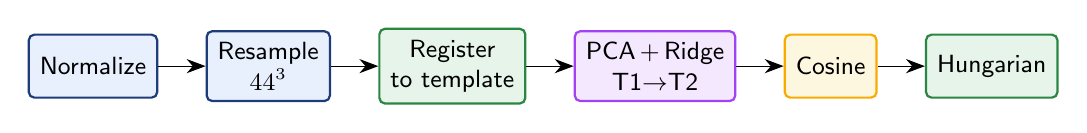
\begin{tikzpicture}[node distance=6mm]
  \node[box] (a) {Normalize};
  \node[box,right=of a] (b) {Resample\\$44^3$};
  \node[greenbox,right=of b] (c) {Register\\to template};
  \node[box,fill=cMathBg,draw=cMathFr,right=of c] (d) {PCA\,+\,Ridge\\T1$\to$T2};
  \node[box,fill=cTradeBg,draw=cTradeFr,right=of d] (e) {Cosine};
  \node[greenbox,right=of e] (f) {Hungarian};
  \draw[->](a)--(b);\draw[->](b)--(c);\draw[->](c)--(d);\draw[->](d)--(e);\draw[->](e)--(f);
\end{tikzpicture}}\par\vspace{14mm}
{\sffamily\large Best public score \textbf{0.920} \quad$\bullet$\quad from a \textbf{0.651} baseline \quad$\bullet$\quad fully classical\par}
\vfill
{\sffamily\small\color{ink!60} A walk through each of the 7 slides, with the reasoning behind every design choice.\par}
\end{titlepage}

\hypersetup{linkcolor=midblue}\tableofcontents\hypersetup{linkcolor=accent}\newpage

This document accompanies the presentation \texttt{EHL\_Paris\_Medical\_Retrieval.pptx}. Each
section below corresponds to one slide and explains, in more depth, \emph{what} is shown and
\emph{why} it works. The whole system is classical --- no neural network, no external data, no
augmentation --- and it climbs from a public score of $0.651$ to $0.920$.

% =====================================================================
\section{Slide 1 --- Title \& headline numbers}
The opening slide states the problem in one line and pins three numbers that frame everything
that follows: the \textbf{best score (0.920)}, the \textbf{starting baseline (0.651)}, and the
\textbf{approach (classical)}.

\textbf{The task.} For each \emph{query} --- a 3D T1 post-contrast brain MRI --- we must rank all
\emph{target} volumes (3D T2 MRI) of a gallery so that the same-subject target sits as high as
possible. It is whole-volume retrieval across two \emph{different} MRI modalities, scored by Mean
Reciprocal Rank (MRR), averaged over three datasets.

\begin{mathidea}[MRR --- the score]
For each query, look at the rank of its true target: rank~1 contributes $1.0$, rank~2 gives
$\tfrac12$, rank~5 gives $\tfrac15$. Average over all queries to get $\mathrm{MRR}_d$ for dataset
$d$; the final score is $\tfrac13(\mathrm{MRR}_1+\mathrm{MRR}_2+\mathrm{MRR}_3)$.
\end{mathidea}

\begin{compression}[The one structural fact we exploit]
In every pool the number of queries equals the number of targets and the matching is
\emph{one-to-one} (a bijection). Retrieval is therefore a \emph{linear assignment problem} --- this
single observation is what later justifies the Hungarian step.
\end{compression}

% =====================================================================
\section{Slide 2 --- Architecture: the retrieval pipeline}
This slide shows the six-stage conveyor that turns a raw NIfTI volume into a ranking. Every volume,
query or target, passes through the same front end; only the geometry handling differs per dataset.

\fitwidth{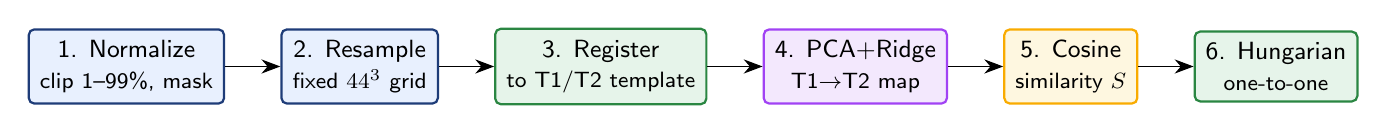
\begin{tikzpicture}[node distance=7mm]
  \node[box] (a) {1. Normalize\\\footnotesize clip 1--99\%, mask};
  \node[box,right=of a] (b) {2. Resample\\\footnotesize fixed $44^3$ grid};
  \node[greenbox,right=of b] (c) {3. Register\\\footnotesize to T1/T2 template};
  \node[box,fill=cMathBg,draw=cMathFr,right=of c] (d) {4. PCA+Ridge\\\footnotesize T1$\to$T2 map};
  \node[box,fill=cTradeBg,draw=cTradeFr,right=of d] (e) {5. Cosine\\\footnotesize similarity $S$};
  \node[greenbox,right=of e] (f) {6. Hungarian\\\footnotesize one-to-one};
  \draw[->](a)--(b);\draw[->](b)--(c);\draw[->](c)--(d);\draw[->](d)--(e);\draw[->](e)--(f);
\end{tikzpicture}}
\figcap{The honest pipeline. Stages 1--2 standardise every volume; 3 puts it in a common frame;
4 bridges the two modalities; 5--6 turn similarities into a one-to-one ranking.}

\begin{system}[Per-dataset switch]
\textbf{d1 \& d2} register to the mean template (their pose differs); \textbf{d2} additionally gets
a \emph{deformable} refinement to undo its elastic warp. \textbf{d3} is already aligned, so it
\emph{skips} registration and uses the raw grid feature. All three end with Hungarian.
\end{system}

\begin{mentalmodel}[The core idea in one sentence]
We \textbf{normalize the distortion away} --- register every volume into one shared coordinate
frame --- instead of training a model to be invariant to it. Removing the nuisance is cheaper and
more reliable than learning to ignore it, especially with only 350 labelled pairs.
\end{mentalmodel}

% =====================================================================
\section{Slide 3 --- Components: why each piece matters}
The slide lists the four load-bearing components. Here is what each one does and the gain it brought.

\subsection{Intensity normalization}
Each volume is masked to the brain, windowed to its 1st--99th intensity percentiles, scaled to
$[0,1]$, and resampled onto a fixed $44\times44\times44$ grid. This makes scans of different dynamic
range comparable and turns every volume into a vector of identical length $44^3$.

\subsection{Template normalization (registration)}
Because d1 pairs are registered, the voxel-wise means $T_1$ and $T_2$ are two \emph{sharp,
mutually-registered} templates. We rigidly align each query to $T_1$ and each target to $T_2$ ---
crucially an \emph{intramodal} alignment (same modality on both sides), which is far more robust
than aligning T1 to T2 directly.

\begin{mathidea}[Why intramodal registration is the trick]
Aligning T1$\leftrightarrow$T1 (or T2$\leftrightarrow$T2) lets us maximise a simple intensity
cross-correlation, which is well-behaved. After both sides land in the shared template frame, the
d1-trained map transfers to d2. Cost is $O(N)$ (one registration per volume), not $O(N^2)$ (every
query--target pair). This single step lifted d1 $0.877\to0.964$ and d2 $0.39\to0.75$.
\end{mathidea}

\subsection{PCA + Ridge cross-modal map}
Query (T1) and target (T2) intensities are not directly comparable. On the 350 labelled pairs we
fit a whitening PCA per modality, then a Ridge regression $W$ that maps query codes into target-code
space. At inference, a query embeds as $u=\mathrm{norm}(W\,P_q\phi^q)$ and a target as
$v=\mathrm{norm}(P_t\phi^t)$; similarity is the cosine $u^\top v$.

\subsection{Deformable (elastic) refinement --- the d2 breakthrough}
Rigid registration removes pose but \emph{not} the nonlinear elastic warp that defines d2. A
regularized Demons deformable registration to the template inverts that residual warp.

\begin{noticethis}[The win that transferred]
Of every modelling idea we tried, deformable registration was the \emph{only} one whose offline
gain carried over to the real leaderboard: $0.904\to0.920$. It works because it attacks the actual
cause of d2's difficulty --- the elastic deformation --- rather than re-ranking around it.
\end{noticethis}

\subsection{Hungarian assignment}
See slide~4's discussion; it converts the global one-to-one matching into per-query rankings.

% =====================================================================
\section{Slide 4 --- Three configurations (the pipeline and two ablations)}
This slide presents the full pipeline next to two ablations, to show how much each structural choice
is worth.

\begin{center}\begin{tabularx}{\textwidth}{@{}l c X@{}}
\toprule
\textbf{Configuration} & \textbf{Score} & \textbf{What changes}\\
\midrule
Full pipeline (best) & \textbf{0.920} & Template + deformable on d2 + Hungarian everywhere.\\
Without deformable & 0.904 & Rigid registration only; d2's elastic warp is left in, so d2 drops from $\approx0.79$ to $\approx0.75$.\\
Without Hungarian & lower & Rank by raw cosine; the bijection is no longer enforced.\\
\bottomrule
\end{tabularx}\end{center}

\begin{mathidea}[What Hungarian actually does]
Given the cosine matrix $S$, we solve $\pi^\star=\arg\max_\pi\sum_i S_{i,\pi(i)}$ with the Hungarian
algorithm (\texttt{linear\_sum\_assignment} on $-S$), then force each query's assigned target to
rank~1 and rank the rest by raw similarity. Because the true matching is a permutation, choosing the
globally consistent assignment fixes many cases where the raw top-1 was a confident impostor.
\end{mathidea}

\begin{tradeoff}[Why removing Hungarian hurts]
Raw cosine ranks each query independently and can assign the same attractive target to several
queries. Hungarian forbids that --- it enforces the one-to-one structure we \emph{know} exists, so
it recovers rank-1 hits that raw scoring misses. Dropping it discards free, certain information.
\end{tradeoff}

% =====================================================================
\section{Slide 5 --- Results: score progression}
The bar chart tells the story of the climb, each step a confirmed Kaggle public score.

\begin{center}\begin{tabularx}{\textwidth}{@{}X c l@{}}
\toprule
\textbf{Step} & \textbf{Score} & \textbf{What it added}\\
\midrule
Canonical baseline & 0.651 & session start\\
+ d2 template normalization & 0.771 & fixes the d2 pose problem\\
+ d1 template & 0.801 & d1 also helped by a common frame\\
+ d3 grid feature (no register) & 0.904 & d3 was being hurt by registration\\
+ d2 deformable registration & 0.919 & inverts d2's elastic warp\\
+ d2 deform + slab fusion (best) & \textbf{0.920} & small extra signal\\
\bottomrule
\end{tabularx}\end{center}

\begin{noticethis}[Offline validation saved submissions]
Kaggle limits submissions and d2/d3 have no labels. We built a \emph{synthetic-d2 harness}: take
labelled d1 pairs, apply independent rigid+elastic warps, and score candidate methods by
Hungarian-recovery MRR. Calibrated so the baseline matches its real d2 score, it ranked methods
\emph{before} we spent a submission --- and correctly predicted the template win.
\end{noticethis}

\begin{misconception}[``A better offline number always means a better real score'']
Not here. Gains that depend on the data \emph{distribution} (higher grid resolution, re-fitting the
map on augmented data, score re-ranking) looked good offline but \emph{regressed} on real data.
Only changes that fix the underlying \emph{geometry} (registration) transferred. We learned to trust
the harness for large structural choices, not small deltas.
\end{misconception}

% =====================================================================
\section{Slide 6 --- What did not work: augmentation}
This slide is deliberately included: it documents a substantial effort that \emph{failed}, so the
result is not repeated. We generated geometric + contrast augmented pairs ($350\to850\to2100$) to
train a second, \emph{learned} model. Every variant made the score worse.

\begin{failure}[What we tried, and the numbers]
\begin{itemize}
\item Contrastive 3D model trained on 850 augmented pairs $\Rightarrow$ holdout MRR $\approx0.04$.
\item Re-fitting the PCA/Ridge map on augmented pairs $\Rightarrow$ d2 $0.749\to0.63$.
\item Real server-side augmentation $\Rightarrow$ d2 $\to0.56$.
\item Fine-tuning a medical foundation network $\Rightarrow$ below the classical pipeline.
\end{itemize}
\end{failure}

\begin{theory}[Why augmentation hurt here]
\textbf{(1) Too few subjects.} Augmentation multiplies \emph{samples} but not \emph{subject
diversity}; 350 distinct brains is too little to learn robust 3D embeddings.
\textbf{(2) Distribution mismatch.} Our synthetic warps do not match d2's real transforms, so any
model or map fitted on them overfits the wrong distribution and degrades on real data.
\textbf{(3) Normalization beats augmentation.} We can \emph{remove} the distortion at inference
(register to a template) instead of teaching a model to tolerate every possible distortion --- a
much smaller, better-posed problem.
\end{theory}

\begin{compression}[The lesson]
When the nuisance transformation is known and invertible (pose, elastic warp), \emph{normalize it
away}. Reserve learned invariance for nuisances you cannot model --- and only when you have the data
to support it.
\end{compression}

% =====================================================================
\section{Slide 7 --- Summary \& takeaways}
The closing slide gives the per-dataset scorecard and the four lessons.

\begin{center}\begin{tabularx}{\textwidth}{@{}l c X@{}}
\toprule
\textbf{Dataset} & \textbf{MRR} & \textbf{Why}\\
\midrule
dataset 1 & $\approx0.96$ & registered; near ceiling\\
dataset 2 & $\approx0.79$ & hardest --- elastic warp, lifted by deformable registration\\
dataset 3 & $\approx1.00$ & already aligned; raw grid feature is near-perfect\\
\bottomrule
\end{tabularx}\end{center}

\begin{compression}[Four takeaways]
\textbf{1.} Exploit structure --- the bijection (Hungarian) and a common frame (registration).\\
\textbf{2.} Deformable registration cracked d2's elastic warp ($+0.016$ on the real board).\\
\textbf{3.} Augmentation hurt; normalization won.\\
\textbf{4.} Validate offline on the synthetic harness before spending a submission.
\end{compression}

From $0.651$ to $0.920$ by pure classical modelling --- no deep learning and no external data.

% =====================================================================
\section{Glossary}
\begin{description}[leftmargin=!,labelwidth=3.2cm,font=\sffamily\bfseries\color{midblue}]
\item[MRI] Magnetic Resonance Imaging.
\item[T1 / T1ce] T1-weighted (post-contrast / ``contrast-enhanced'') MRI --- the query modality.
\item[T2] T2-weighted MRI --- the target modality.
\item[MRR] Mean Reciprocal Rank --- the competition metric.
\item[NIfTI] The 3D medical-image file format used for the volumes.
\item[Bijection] A one-to-one correspondence; here, each query has exactly one true target.
\item[PCA] Principal Component Analysis --- whitening / dimensionality reduction per modality.
\item[Ridge] $L_2$-regularized linear regression --- learns the T1$\to$T2 code map.
\item[Template normalization] Registering each volume to a mean (template) brain of its modality.
\item[Rigid registration] Alignment by rotation + translation only (6 parameters).
\item[Deformable / elastic registration] Alignment with a dense per-voxel displacement field; can
undo nonlinear warps.
\item[Demons] A classical deformable-registration algorithm (used via SimpleITK).
\item[NCC] Normalized Cross-Correlation --- the intramodal registration similarity metric.
\item[Hungarian algorithm] Solves the optimal one-to-one assignment of a cost matrix.
\item[Harness] Our offline synthetic-d2 validator built from labelled d1 pairs.
\end{description}

\end{document}
